\documentclass{beamer}

\usepackage{comment}
\usepackage{color}
\usepackage{listings}
\usepackage{verbatim}
\usepackage{multicol}
\usepackage{booktabs}
\definecolor{green}{RGB}{0,128,0}

\def\EQ#1\EN{\begin{equation*}#1\end{equation*}}
\def\BA#1\EA{\begin{align*}#1\end{align*}}
\def\BS#1\ES{\begin{split*}#1\end{split*}}
\newcommand{\bc}{\begin{center}}
\newcommand{\ec}{\end{center}}
\newcommand{\eq}{\ =\ }

\newcommand\p{\partial}
\newcommand\gD{\mathcal D}
\newcommand{\bnabla}{\boldsymbol{\nabla}}
\newcommand{\bq}{\boldsymbol{q}}
\newcommand{\bOmega}{\boldsymbol{\Omega}}

\def\Li{\textit{L}}
\def\Fb{\textbf{f}}
\def\Jb{\textbf{J}}
\def\cb{\textbf{c}}

\newcommand{\caq}{c_\text{aq}}
\newcommand{\csb}{c_\text{sb}}
\newcommand{\kd}{k_D}

\newcommand\gehcomment[1]{{{\color{orange} #1}}}
\newcommand\add[1]{{{\color{blue} #1}}}
\newcommand\remove[1]{\sout{{\color{red} #1}}}
\newcommand\codecomment[1]{{{\color{green} #1}}}
\newcommand\redcomment[1]{{{\color{red} #1}}}
\newcommand\bluecomment[1]{{{\color{blue} #1}}}
\newcommand\greencomment[1]{{{\color{green} #1}}}
\newcommand\magentacomment[1]{{{\color{magenta} #1}}}

\begin{comment}
\tiny
\scriptsize
\footnotesize
\small
\normalsize
\large
\Large
\LARGE
\huge
\Huge
\end{comment}

\begin{document}
\title{1D Transport, Sorption and Decay Scenario\ldots\\in a Nutshell}
\author{Glenn Hammond}
\date{\today}

\frame{\titlepage}

% enable breaks within frame
%\begin{frame}[fragile,containsverbatim,allowframebreaks]\frametitle{Frame Title}

%-----------------------------------------------------------------------------
\section{Description of 1D Transport, Sorption and Decay Scenario}

\frame{\frametitle{Description of 1D Transport, Sorption and Decay Scenario}

\begin{figure}
\centering
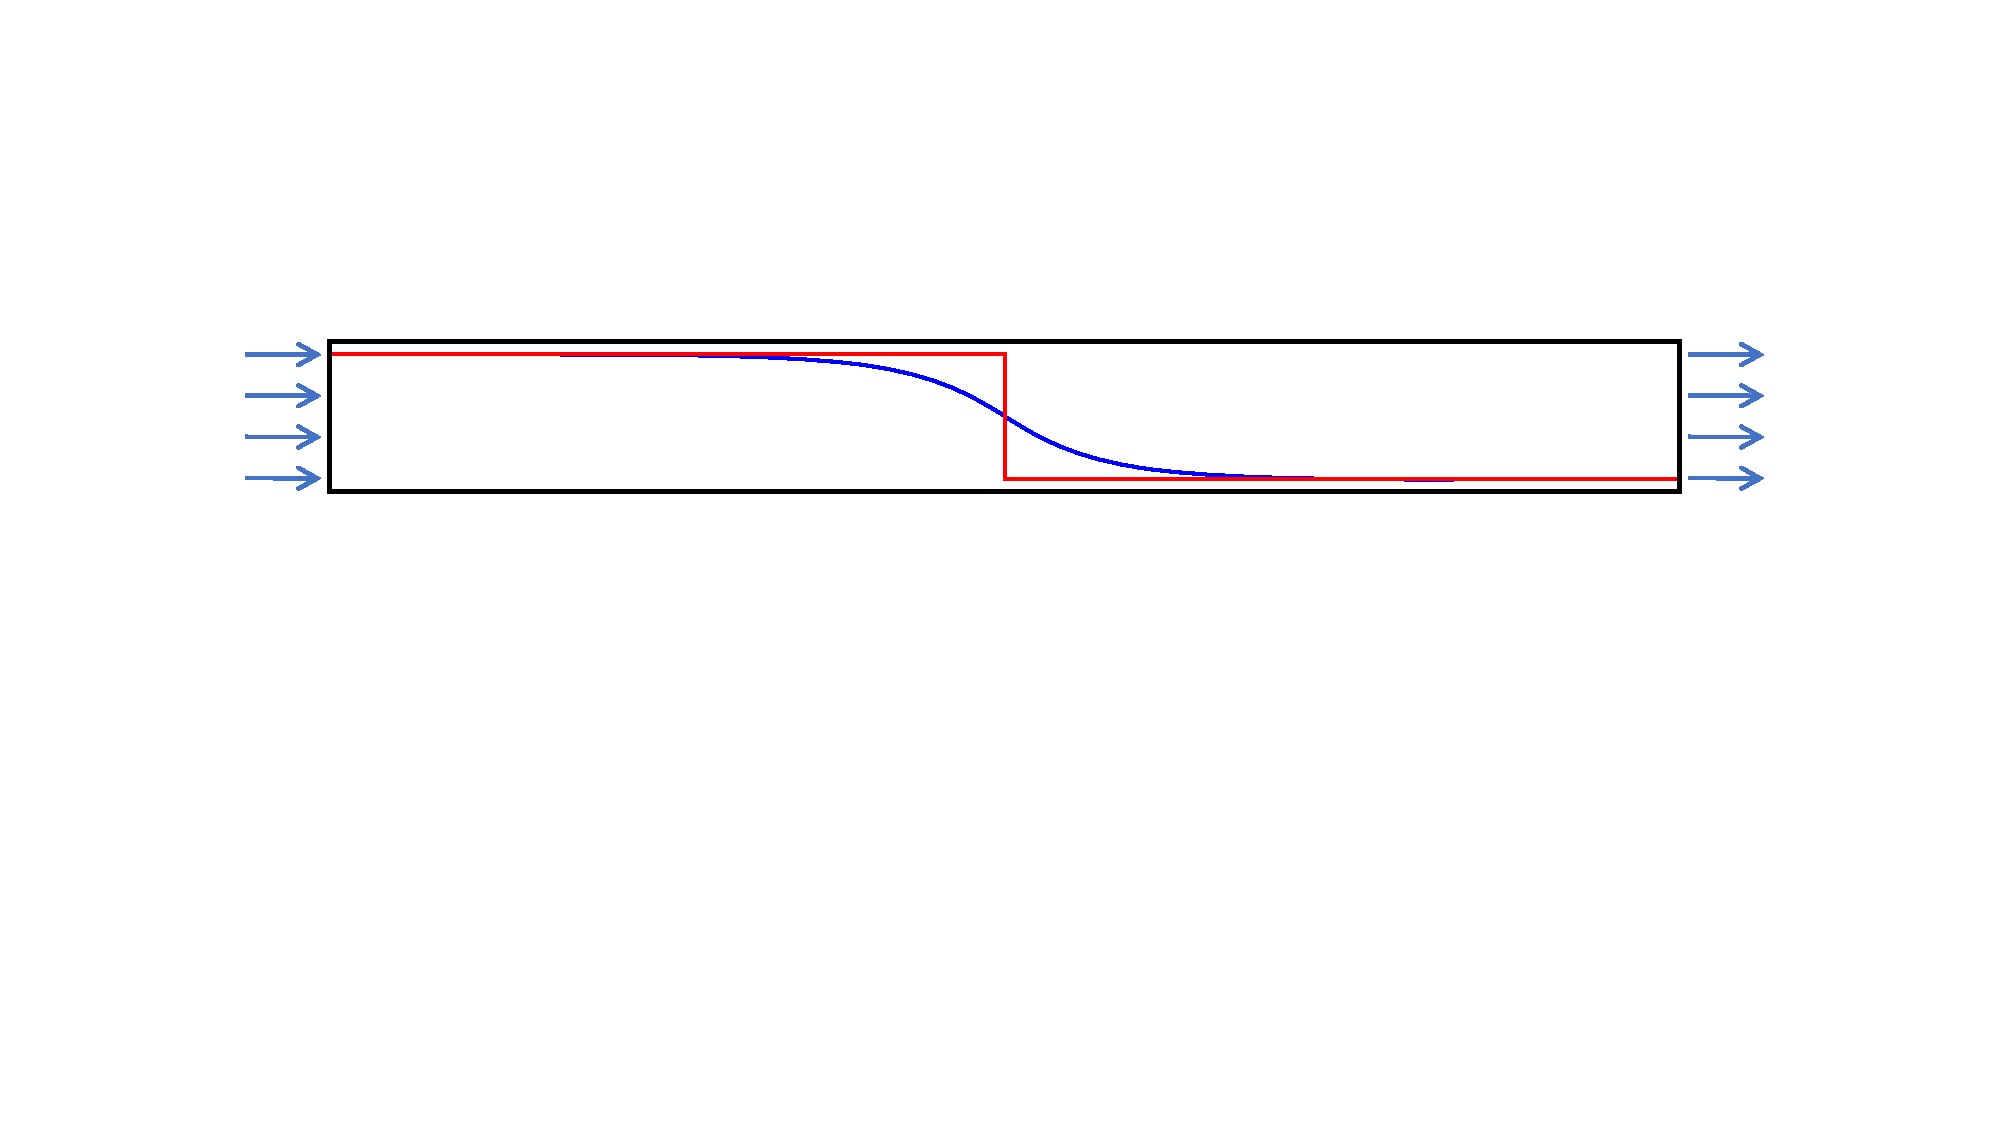
\includegraphics[width=0.9\linewidth]{./advection_dispersion_fig}
\end{figure}
The ``1D Transport, Sorption and Decay Scenario'' simulates solute transport (i.e., advection and diffusion), linear sorption and radioactive decay along a horizontal, 1D domain measuring 100 meters in length with unit cross sectional area.  Assumptions regarding transport include:

\begin{itemize}
  \item Problem domain: $100 \times 1 \times 1$ m (x $\times$ y $\times$ z)
  \item Grid resolution $1 \times 1 \times 1$ m
  \item Darcy flow velocity: 1 m/y (left to right or west to east)
  \item Porosity: 0.25
  \item Maximum time step size: 0.25 y (CFL = 1.)
  \item Total simulation time: 25 y
\end{itemize}

}

%-----------------------------------------------------------------------------
\frame{\frametitle{Governing Reactive Transport Equations}

\Large

\EQ\label{trans}
\frac{\p}{\p t} \left(\phi s\,\caq + \csb\right) + \bnabla\cdot\bOmega \eq -k\left(\phi s\,\caq + \csb\right)
\EN

\EQ\label{flux}
\bOmega \eq \big(\bq - \phi s \tau \gD\bnabla\big) \caq
\EN

%\bigskip
%\normalsize
\footnotesize
\begin{align*}
\phi &\eq \text{porosity}; \quad
s \eq \text{liquid saturation}; \quad
\tau \eq \text{tortuosity} \\
\caq &\eq \text{aqueous concentration}\\
\csb &\eq \text{sorbed concentration} \eq \kd\,\caq \\
\kd &\eq \text{distribution coefficient} \\
\bOmega &\eq \text{solute flux} \\
\bq &\eq \text{Darcy velocity} \\
\gD &\eq \text{coefficient of diffusion}\\
k &\eq \text{first-order rate constant}
\end{align*}

}

%-----------------------------------------------------------------------------
\section{Description of Input Deck: Transport Only}

\begin{frame}[fragile]\frametitle{Transport Only}

\Large
Set up the input file.
\large
\begin{itemize}
  \item Add SIMULATION block
  \item Add SUBSURFACE block
\end{itemize}

\end{frame}

%-----------------------------------------------------------------------------
\begin{frame}[fragile]\frametitle{SIMULATION}

\begin{itemize}
  \item Specify subsurface simulation
  \item Specify the use of the transport process model
\end{itemize}


\begin{semiverbatim}

SIMULATION
  SIMULATION_TYPE SUBSURFACE
  PROCESS_MODELS
    SUBSURFACE_TRANSPORT transport \bluecomment{! process model name}
      MODE GIRT   \bluecomment{! \redcomment{G}lobal \redcomment{I}mplicit \redcomment{R}eactive \redcomment{T}ransport}
    /
  /
END

SUBSURFACE
  ...
END_SUBSURFACE
\end{semiverbatim}

\end{frame}

%-----------------------------------------------------------------------------
\begin{frame}[fragile,containsverbatim]\frametitle{GRID}

\begin{itemize}
  \item Problem domain: $100 \times 1 \times 1$ m (x $\times$ y $\times$ z)
  \item Grid resolution $1 \times 1 \times 1$ m
\end{itemize}

\begin{semiverbatim}
GRID
  TYPE STRUCTURED     \bluecomment{! structured grid}
  NXYZ 100 1 1        \bluecomment{! NX, NY, NZ}
  BOUNDS              \bluecomment{! define the rectangular domain}
    0. 0. 0.          \bluecomment{! xmin ymin zmin}
    100. 1. 1.        \bluecomment{! xmax ymax zmax}
  /  \bluecomment{! <-- closes out BOUNDS card}
END  \bluecomment{! <-- closes out GRID card}
\end{semiverbatim}

\end{frame}

%-----------------------------------------------------------------------------
\begin{frame}[fragile,containsverbatim,allowframebreaks]\frametitle{REGION}

\vspace{1 cm}
\begin{itemize}
  \item Delineate regions in the 1D domain for:
  \begin{itemize}
    \item west boundary face
    \item east boundary face
    \item entire domain (all)
  \end{itemize}
\end{itemize}

\begin{semiverbatim}

REGION all            \bluecomment{! define a region and name it: \greencomment{all}}
  COORDINATES         \bluecomment{! using \redcomment{volumetric} coordinates}
    0. 0. 0.          \bluecomment{! lower coordinate: xmin ymin zmin}
    100. 1. 1.        \bluecomment{! upper coordinate: xmax ymax zmax}
  /   \bluecomment{! <-- closes out COORDINATES card}
END   \bluecomment{! <-- closes out REGION card}

\newpage
REGION west           \bluecomment{! define region:} \greencomment{west}
  FACE WEST           \bluecomment{! define the face of the grid cell}
  COORDINATES         \bluecomment{! using \redcomment{surface} coordinates}
    0. 0. 0.
    0. 1. 1.
  /
END

REGION east           \bluecomment{! define region:} \greencomment{east}
  FACE EAST           \redcomment{! WEST, EAST, SOUTH, NORTH,}
  COORDINATES         \redcomment{!   BOTTOM, TOP} \bluecomment{ are keywords}
    100. 0. 0.        \bluecomment{!   in PFLOTRAN.}
    100. 1. 1.
  /
END

\end{semiverbatim}

\end{frame}

%-----------------------------------------------------------------------------
\begin{frame}[fragile,containsverbatim]\frametitle{MATERIAL\_PROPERTY}

\begin{itemize}
  \item Define a soil with:
  \begin{itemize}
    \item Material id = 1
    \item Porosity = 0.25
    \item Tortuosity = 1.
  \end{itemize}
\end{itemize}

\begin{semiverbatim}


MATERIAL_PROPERTY soil1  \bluecomment{! user-defined name}
  ID 1                   \bluecomment{! All grid cells of this}
  POROSITY 0.25          \bluecomment{!   material type will have}
  TORTUOSITY 1.          \bluecomment{!   a material \redcomment{ID = 1}.}
END
\end{semiverbatim}

\end{frame}

%-----------------------------------------------------------------------------
\begin{frame}[fragile,containsverbatim]\frametitle{FLUID\_PROPERTY}

\begin{itemize}
  \item Assign a molecular diffusion coefficient of $10^{-8}$ m$^2$/s to all aqueous species
\end{itemize}

\begin{semiverbatim}

FLUID_PROPERTY                  \bluecomment{! fluid is water}
  DIFFUSION_COEFFICIENT 1.d-8   \bluecomment{! [m^2/s]}
END
\end{semiverbatim}

\end{frame}

%-----------------------------------------------------------------------------
\begin{frame}[fragile]\frametitle{CHEMISTRY}

\begin{itemize}
  \item One primary species: Aaq
\end{itemize}

\begin{semiverbatim}
CHEMISTRY
  PRIMARY_SPECIES
    Aaq
  /
  OUTPUT
    TOTAL        \bluecomment{! total component concentration}
    ALL          \bluecomment{! for all species}
  /
END
\end{semiverbatim}

\end{frame}

%-----------------------------------------------------------------------------
\begin{frame}[fragile]\frametitle{CONSTRAINT}

\begin{itemize}
  \item Set up molarity concentration constraints for boundary and initial conditions
\end{itemize}

\begin{semiverbatim}

CONSTRAINT initial_constraint \bluecomment{! user-defined name}
  CONCENTRATIONS
    Aaq   1.d-10   T
  /      \bluecomment{! T = total component concentration [M]}
END

CONSTRAINT inlet_constraint
  CONCENTRATIONS
    Aaq   1.d-3    T
  /
END

\end{semiverbatim}

\end{frame}

%-----------------------------------------------------------------------------
\begin{frame}[fragile]\frametitle{TRANSPORT\_CONDITION}


\begin{itemize}
  \item Couple transport constraints with transport conditions
\end{itemize}
\begin{semiverbatim}
TRANSPORT_CONDITION background_conc \bluecomment{! user-defined name}
  TYPE ZERO_GRADIENT
  CONSTRAINT_LIST
    \bluecomment{! list has to begin at time = \redcomment{0.}}
    0. initial_constraint
  /
END

TRANSPORT_CONDITION inlet_conc
  TYPE DIRICHLET_ZERO_GRADIENT
  CONSTRAINT_LIST
    0. inlet_constraint
  /
END
\end{semiverbatim}

\end{frame}

%-----------------------------------------------------------------------------
\begin{frame}[fragile]\frametitle{STRATA}

\begin{itemize}
\item Couple \greencomment{soil1} rock/soil type with region \greencomment{all} to define a stratigraphic unit
\end{itemize}

\begin{semiverbatim}

STRATA
  REGION all
  MATERIAL soil1
END


\end{semiverbatim}

\end{frame}

%-----------------------------------------------------------------------------
\begin{frame}[fragile]\frametitle{INITIAL\_CONDITION}

\begin{itemize}
\item Couple the \greencomment{initial} transport condition with region \greencomment{all} for the initial condition
\end{itemize}

\begin{semiverbatim}

INITIAL_CONDITION          \bluecomment{! notice: no name}
  TRANSPORT_CONDITION background_conc
  REGION all
END

\end{semiverbatim}

\end{frame}

%-----------------------------------------------------------------------------
\begin{frame}[fragile]\frametitle{BOUNDARY\_CONDITION}

\begin{itemize}
\item Couple the \greencomment{inlet\_conc} transport condition with region \greencomment{west} for the \redcomment{inlet} boundary condition.
\item Couple the \greencomment{background\_conc} transport condition with region \greencomment{east} for the \redcomment{outlet} boundary condition.
\end{itemize}

\begin{semiverbatim}

BOUNDARY_CONDITION outlet     \bluecomment{! name is recommended}
  TRANSPORT_CONDITION background_conc
  REGION east
END

BOUNDARY_CONDITION inlet
  TRANSPORT_CONDITION inlet_conc
  REGION west
END

\end{semiverbatim}

\end{frame}

%-----------------------------------------------------------------------------
\begin{frame}[fragile]\frametitle{LINEAR\_SOLVER}

\begin{itemize}
\item Due to the small problem size, request a direct solver instead of the default iterative BiCGStab Krylov solver.
\end{itemize}

\begin{semiverbatim}

NUMERICAL_METHODS TRANSPORT
  LINEAR_SOLVER
    SOLVER DIRECT
  /
END

\end{semiverbatim}

\end{frame}

%-----------------------------------------------------------------------------
\begin{frame}[fragile]\frametitle{TIME}

\begin{itemize}
\item Set final simulation time to 25 years
\item Set initial time step size to 1. h
\item Set maximum time step size to 0.25 years
\end{itemize}


\begin{semiverbatim}

TIME
  FINAL_TIME 25. \redcomment{y}      \bluecomment{! time units converted to SI [s]}
  INITIAL_TIMESTEP_SIZE 1. \redcomment{h}
  MAXIMUM_TIMESTEP_SIZE 0.25 \redcomment{y}
END
\end{semiverbatim}

\end{frame}

%-----------------------------------------------------------------------------
\begin{frame}[fragile]\frametitle{OUTPUT}

\begin{itemize}
\item Specify output times (5, 10, 15, 20 years) and format (Tecplot point datapacking).
\item The initial and final simulation times are automatically added to the list of output times.
\item Note that additional output options (e.g. species names) are specified within CHEMISTRY.
\end{itemize}


\begin{semiverbatim}

OUTPUT
  TIMES \redcomment{y} 5. 10. 15. 20.
  FORMAT TECPLOT POINT
END
\end{semiverbatim}

\end{frame}

%-----------------------------------------------------------------------------
\begin{frame}[fragile]\frametitle{Flow Field}

\begin{itemize}
\item Specify a uniform Darcy velocity of 1 m/y in x-direction
\item Specify a uniform liquid densify of 1000 kg/m$^3$
\end{itemize}


\begin{semiverbatim}

SPECIFIED_VELOCITY
  UNIFORM? YES
  DATASET 1. 0. 0. m/yr
END

REFERENCE_LIQUID_DENSITY 1000. kg/m^3
\end{semiverbatim}

\end{frame}

%-----------------------------------------------------------------------------
\begin{frame}[fragile]\frametitle{Running PFLOTRAN}

\begin{semiverbatim}

> cd $PFLOTRAN_DIR
> cd shortcourse/exercises/1D_sorption_decay
> pflotran -input_prefix transport
> python plot_transport.py

\end{semiverbatim}

\end{frame}

%-----------------------------------------------------------------------------
\section{Description of Input Deck: Transport and Sorption}

\begin{frame}[fragile]\frametitle{Transport and Sorption}

Input File Modifications
\begin{itemize}
\item Modify cards:
  \begin{itemize}
    \item CHEMISTRY
    \item CONSTRAINT
    \item MATERIAL\_PROPERTY
   \end{itemize}
\item Add cards:
  \begin{itemize}
    \item SORPTION
  \end{itemize}
\end{itemize}

\end{frame}

%-----------------------------------------------------------------------------
\begin{frame}[fragile,containsverbatim,allowframebreaks]\frametitle{CHEMISTRY}

\begin{itemize}
  \item Add primary species Baq
  \item Add geochemistry database
  \item Specify \verb|LOG_FORMULATION| to improve solver convergence
\end{itemize}

\begin{semiverbatim}
CHEMISTRY
  PRIMARY_SPECIES
    Aaq
    \magentacomment{Baq}
  /
  \magentacomment{DATABASE ../../../database/simple_rxn_database.dat}
  \magentacomment{LOG_FORMULATION}
  OUTPUT
    TOTAL
    ALL
  /
END
\end{semiverbatim}

\end{frame}

%-----------------------------------------------------------------------------
\begin{frame}[fragile,containsverbatim]\frametitle{MATERIAL\_PROPERTY}

\begin{itemize}
  \item Add soil particle density = 2650. kg/m$^3$
\end{itemize}

\begin{semiverbatim}

MATERIAL_PROPERTY soil1
  ID 1
  POROSITY 0.25
  TORTUOSITY 1.
  \magentacomment{ROCK_DENSITY 2650. kg/m^3}
END

\end{semiverbatim}

\end{frame}

%-----------------------------------------------------------------------------
\begin{frame}[fragile]\frametitle{CONSTRAINT}

\begin{itemize}
  \item Add concentrations for Baq
\end{itemize}

\begin{semiverbatim}

CONSTRAINT initial_constraint
  CONCENTRATIONS
    Aaq   1.d-10   T
    \magentacomment{Baq   1.d-10   T}
  /
END

CONSTRAINT inlet_constraint
  CONCENTRATIONS
    Aaq   1.d-3    T
    \magentacomment{Baq   1.d-3    T}
  /
END

\end{semiverbatim}

\end{frame}

%-----------------------------------------------------------------------------
\begin{frame}[fragile,containsverbatim,allowframebreaks]\frametitle{SORPTION}

\begin{itemize}
  \item Add linear sorption reaction
\end{itemize}

\begin{semiverbatim}
CHEMISTRY
  ...
  \magentacomment{SORPTION}
    \magentacomment{ISOTHERM_REACTIONS}
      \magentacomment{Baq}
        \magentacomment{TYPE LINEAR}
        \bluecomment{# Retardation (R) as a function of distribution coefficient (Kd):}
        \bluecomment{#   R = 1+bulk_rock_density*Kd/porosity}
        ...
        \magentacomment{DISTRIBUTION_COEFFICIENT 1.25786d-4 m^3/kg}
      \magentacomment{/}
    \magentacomment{/}
  \magentacomment{/}
  ...
END
\end{semiverbatim}

\end{frame}

%-----------------------------------------------------------------------------
\begin{frame}[fragile]\frametitle{Running PFLOTRAN}

\begin{semiverbatim}

> cd $PFLOTRAN_DIR
> cd shortcourse/exercises/1D_sorption_decay
> pflotran -input_prefix transport_sorption
> python plot_transport_sorption.py

\end{semiverbatim}

\end{frame}

%-----------------------------------------------------------------------------
\section{Description of Input Deck: Transport and Radioactive Decay}

\begin{frame}[fragile]\frametitle{Transport and Radioactive Decay}

Input File Modifications (beginning with \textit{transport.in})
\begin{itemize}
\item Modify cards:
  \begin{itemize}
    \item CHEMISTRY
    \item CONSTRAINT
   \end{itemize}
\item Add cards:
  \begin{itemize}
    \item RADIOACTIVE\_DECAY\_REACTION
  \end{itemize}
\end{itemize}

\end{frame}

%-----------------------------------------------------------------------------
\begin{frame}[fragile,containsverbatim,allowframebreaks]\frametitle{CHEMISTRY}

\begin{itemize}
  \item Add primary species Caq and Daq
  \item Add geochemistry database
  \item Specify \verb|LOG_FORMULATION| to improve solver convergence
\end{itemize}

\begin{semiverbatim}
CHEMISTRY
  PRIMARY_SPECIES
    Aaq
    \magentacomment{Caq}
    \magentacomment{Daq}
  /
  \magentacomment{DATABASE ../../../database/simple_rxn_database.dat}
  \magentacomment{LOG_FORMULATION}
  OUTPUT
    TOTAL
    ALL
  /
END
\end{semiverbatim}

\end{frame}

%-----------------------------------------------------------------------------
\begin{frame}[fragile]\frametitle{CONSTRAINT}

\begin{itemize}
  \item Add concentrations for Baq
\end{itemize}

\begin{semiverbatim}

CONSTRAINT initial_constraint
  CONCENTRATIONS
    Aaq   1.d-10   T
    \magentacomment{Caq   1.d-10   T}
    \magentacomment{Daq   1.d-10   T}
  /
END

CONSTRAINT inlet_constraint
  CONCENTRATIONS
    Aaq   1.d-3    T
    \magentacomment{Caq   1.d-3    T}
    \magentacomment{Daq   1.d-10   T}
  /
END

\end{semiverbatim}

\end{frame}

%-----------------------------------------------------------------------------
\begin{frame}[fragile,containsverbatim,allowframebreaks]\frametitle{RADIOACTIVE\_DECAY\_REACTION}

\begin{itemize}
  \item Add radioactive decay reaction
\end{itemize}

\begin{semiverbatim}

CHEMISTRY
  ...
  \magentacomment{RADIOACTIVE_DECAY_REACTION}
    \bluecomment{# Calculating rate constant (k) from half life:}
    \bluecomment{#   k = -ln(0.5)/half_life}
    \bluecomment{# For half_life = 10 y.:}
    \bluecomment{#   k = 0.0693147... = -ln(0.5)/10}
    \bluecomment{# Use half life instead}
    \magentacomment{REACTION Caq -> Daq}
    \magentacomment{RATE_CONSTANT 0.0693147 1/y}
  \magentacomment{/}
  ...
END
\end{semiverbatim}

\end{frame}

%-----------------------------------------------------------------------------
\begin{frame}[fragile]\frametitle{Running PFLOTRAN}

\begin{semiverbatim}

> cd $PFLOTRAN_DIR
> cd shortcourse/exercises/1D_sorption_decay
> pflotran -input_prefix transport_decay
> python plot_transport_decay.py

\end{semiverbatim}

\end{frame}

%-----------------------------------------------------------------------------
\section{Description of Input Deck: Transport, Sorption and Radioactive Decay}

\begin{frame}[fragile]\frametitle{Transport, Sorption and Radioactive Decay}

Input File Modifications (beginning with a merge of \textit{transport\_sorption.in} and \textit{transport\_decay.in})
\begin{itemize}
\item Modify cards:
  \begin{itemize}
    \item CHEMISTRY
    \item CONSTRAINT
    \item SORPTION
   \end{itemize}
\item Add cards:
  \begin{itemize}
    \item RADIOACTIVE\_DECAY\_REACTION
  \end{itemize}
\end{itemize}

\end{frame}

%-----------------------------------------------------------------------------
\begin{frame}[fragile]\frametitle{CHEMISTRY}

\begin{itemize}
  \item Add primary species Eaq and Faq
\end{itemize}

\begin{semiverbatim}
CHEMISTRY
  PRIMARY_SPECIES
    Aaq
    Baq
    Caq
    Daq
    \magentacomment{Eaq}
    \magentacomment{Faq}
  /
  ...
  OUTPUT
    TOTAL
    ALL
  /
END
\end{semiverbatim}

\end{frame}

%-----------------------------------------------------------------------------
\begin{frame}[fragile]\frametitle{CONSTRAINT}

\begin{itemize}
  \item Add concentrations for Eaq and Faq
\end{itemize}

\begin{semiverbatim}
CONSTRAINT initial_constraint
  CONCENTRATIONS
    ...
    \magentacomment{Eaq   1.d-10   T}
    \magentacomment{Faq   1.d-10   T}
  /
END

CONSTRAINT inlet_constraint
  CONCENTRATIONS
    ...
    \magentacomment{Eaq   1.d-3    T}
    \magentacomment{Faq   1.d-10   T}
  /
END
\end{semiverbatim}

\end{frame}

%-----------------------------------------------------------------------------
\begin{frame}[fragile]\frametitle{SORPTION and RADIOACTIVE\_DECAY\_REACTION}

\begin{itemize}
  \item Add sorption and radioactive decay reactions
\end{itemize}

\begin{semiverbatim}
CHEMISTRY
  ...
  SORPTION
    ISOTHERM_REACTIONS
      ...
      \magentacomment{Eaq}
        \magentacomment{TYPE LINEAR}
        \magentacomment{DISTRIBUTION_COEFFICIENT 1.25786d-4 m^3/kg}
      \magentacomment{/}
    /
  /
  \magentacomment{RADIOACTIVE_DECAY_REACTION}
    \magentacomment{REACTION Eaq -> Faq}
    \magentacomment{HALF_LIFE 10. y}
  \magentacomment{/}
  ...
\end{semiverbatim}

\end{frame}

%-----------------------------------------------------------------------------
\begin{frame}[fragile]\frametitle{Running PFLOTRAN}

\begin{semiverbatim}

> cd $PFLOTRAN_DIR
> cd shortcourse/exercises/1D_sorption_decay
> pflotran -input_prefix transport_sorption_decay
> python plot_transport_sorption_decay.py

\end{semiverbatim}

\end{frame}

\end{document}
